\documentclass{article}
\usepackage{graphicx} 
\usepackage{hyperref}

\title{Advanced programming for HPC - Labwork 5}
\author{Son Dang Thai}
\date{October 2025}

\begin{document}

\maketitle

\section{Implementation}
This labwork was carried out on a 512x512 image

\begin{figure}[!htb]
    \begin{minipage}{0.48\textwidth}
        \centering
        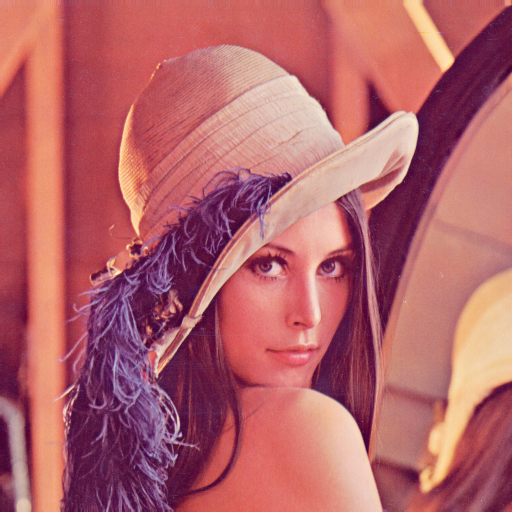
\includegraphics[width=.7\linewidth]{lenna.png}
        \caption{Experiment photo}
        \label{fig:rgb}
    \end{minipage}\hfill
    \begin{minipage}{0.48\textwidth}
        \centering
        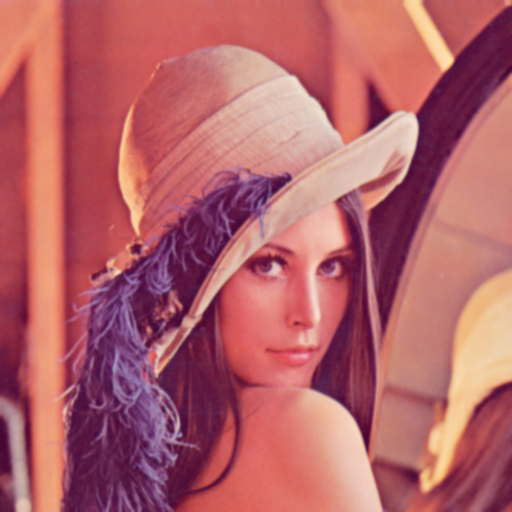
\includegraphics[width=.7\linewidth]{lenna_blur_with_shared.png}
        \caption{Blur result}
        \label{fig:blur}
    \end{minipage}\hfill
\end{figure}

Generally, to use the Gaussian blur convolution, after copying the image and the filter to GPU, the kernel is applied to every pixel in the image. Each new pixel value is calculated as a weighted average of its neighboring pixels, with weights determined by the corresponding values in the kernel. 

Therefore, in the main function using the global memory, there is a 2-nested loop over the coordination x and y of each pixel in the image calculating the new RGB values.

The difference in the function using the shared memory is that before the main 2-nested loop, an empty grid of the same size as the filter is created in the shared memory. Then, a small loop is used to copy the all the filter information to that empty grid for each block: starting from the current local thread’s ID of a block, increasing by the total number of threads in the block, until reaching the total number of elements. After this, everything stays the same except that the filter is retrieved from the shared memory.

\section{Response time}

Below is the response time graph:

\begin{figure}[!htb]
    \begin{minipage}{0.48\textwidth}
        \centering
        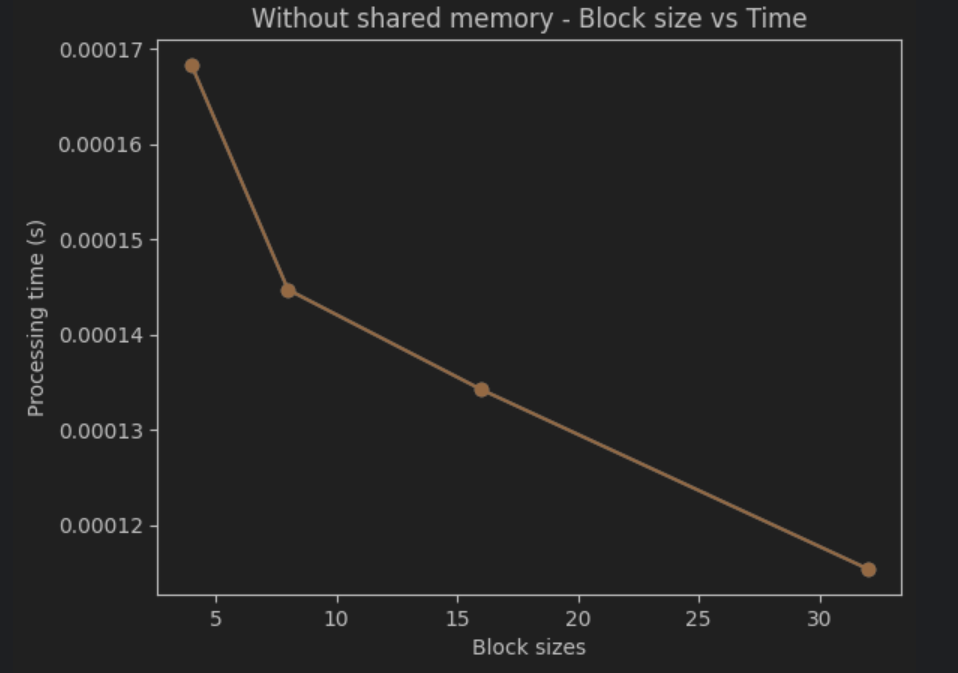
\includegraphics[width=.7\linewidth]{Without shared memory - Block size vs Time.png}
        \caption{Without shared memory}
        \label{fig:1D Without shared memory}
    \end{minipage}\hfill
    \begin{minipage}{0.48\textwidth}
        \centering
        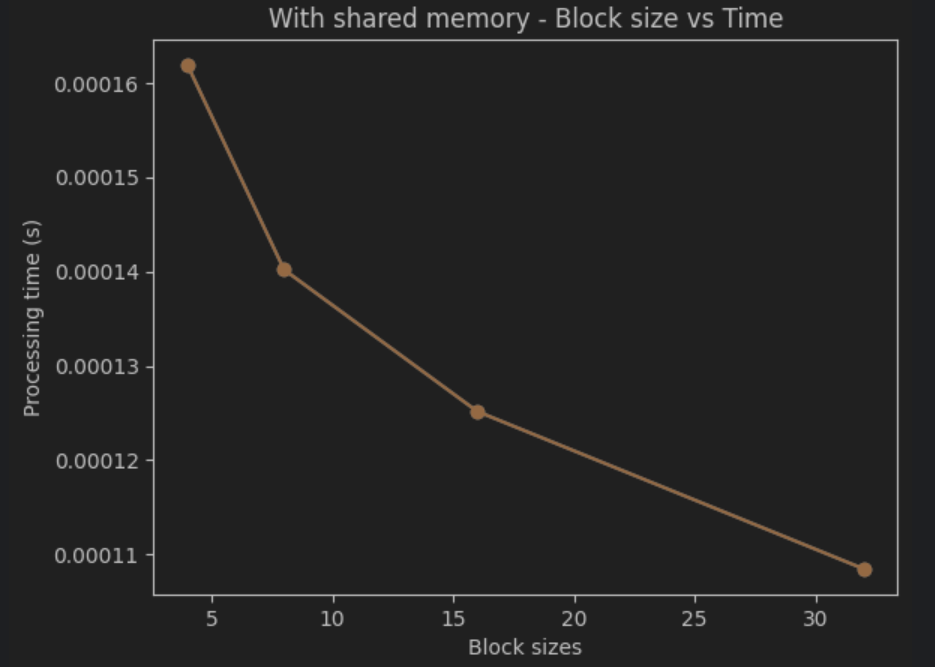
\includegraphics[width=.7\linewidth]{With shared memory - Response time according to block size.png}
        \caption{With shared memory}
        \label{fig:2D With shared memory}
    \end{minipage}\hfill
\end{figure}

Without the shared memory, with block sizes [(4, 4), (8, 8), (16, 16), (32, 32)], the resposne time was recorded at [0.00016832351684570312, 0.00014472007751464844, 0.0001342296600341797, 0.00011539459228515625] seconds.

With the shared memory, with block sizes [(4, 4), (8, 8), (16, 16), (32, 32)], the resposne time was recorded at [0.00016188621520996094, 0.00014019012451171875, 0.0001251697540283203, 0.00010848045349121094] seconds.

This shows that using the shared memory in this labwork makes the work a little bit faster, and the larger the block size, the shorter the response time.

\end{document}
